\documentclass[10pt]{article}


\usepackage[a4paper , left=31.7mm, top=25.4mm]{geometry}


\usepackage{hyperref}
\hypersetup{
	colorlinks=true,
    linkcolor=blue,
    filecolor=magenta,      
    urlcolor=cyan,
    pdftitle={Overleaf Example}
}

\setlength\parindent{0pt}
\usepackage{listings}
% Copyright 2017 Sergei Tikhomirov, MIT License
% https://github.com/s-tikhomirov/solidity-latex-highlighting/

\usepackage{listings, xcolor}

\definecolor{verylightgray}{rgb}{.97,.97,.97}

\lstdefinelanguage{Solidity}{
	keywords=[1]{anonymous, assembly, assert, balance, break, call, callcode, case, catch, class, constant, continue, constructor, contract, debugger, default, delegatecall, delete, do, else, emit, event, experimental, export, external, false, finally, for, function, gas, if, implements, import, in, indexed, instanceof, interface, internal, is, length, library, log0, log1, log2, log3, log4, memory, modifier, new, payable, pragma, private, protected, public, pure, push, require, return, returns, revert, selfdestruct, send, solidity, storage, struct, suicide, super, switch, then, this, throw, transfer, true, try, typeof, using, value, view, while, with, addmod, ecrecover, keccak256, mulmod, ripemd160, sha256, sha3}, % generic keywords including crypto operations
	keywordstyle=[1]\color{blue}\bfseries,
	keywords=[2]{address, bool, byte, bytes, bytes1, bytes2, bytes3, bytes4, bytes5, bytes6, bytes7, bytes8, bytes9, bytes10, bytes11, bytes12, bytes13, bytes14, bytes15, bytes16, bytes17, bytes18, bytes19, bytes20, bytes21, bytes22, bytes23, bytes24, bytes25, bytes26, bytes27, bytes28, bytes29, bytes30, bytes31, bytes32, enum, int, int8, int16, int24, int32, int40, int48, int56, int64, int72, int80, int88, int96, int104, int112, int120, int128, int136, int144, int152, int160, int168, int176, int184, int192, int200, int208, int216, int224, int232, int240, int248, int256, mapping, string, uint, uint8, uint16, uint24, uint32, uint40, uint48, uint56, uint64, uint72, uint80, uint88, uint96, uint104, uint112, uint120, uint128, uint136, uint144, uint152, uint160, uint168, uint176, uint184, uint192, uint200, uint208, uint216, uint224, uint232, uint240, uint248, uint256, var, void, ether, finney, szabo, wei, days, hours, minutes, seconds, weeks, years},	% types; money and time units
	keywordstyle=[2]\color{teal}\bfseries,
	keywords=[3]{block, blockhash, coinbase, difficulty, gaslimit, number, timestamp, msg, data, gas, sender, sig, value, now, tx, gasprice, origin},	% environment variables
	keywordstyle=[3]\color{violet}\bfseries,
	identifierstyle=\color{black},
	sensitive=false,
	comment=[l]{//},
	morecomment=[s]{/*}{*/},
	commentstyle=\color{gray}\ttfamily,
	stringstyle=\color{red}\ttfamily,
	morestring=[b]',
	morestring=[b]"
}

\lstset{
	language=Solidity,
	backgroundcolor=\color{verylightgray},
	extendedchars=true,
	basicstyle=\footnotesize\ttfamily,
	showstringspaces=false,
	showspaces=false,
	numbers=left,
	numberstyle=\footnotesize,
	numbersep=9pt,
	tabsize=2,
	breaklines=true,
	showtabs=false,
	captionpos=b
}

\usepackage{tikz}
\usetikzlibrary{shapes.geometric , arrows}

%tikzlibrary

\tikzstyle{startstop} = [rectangle, rounded corners, minimum width=3cm, minimum height=0.6cm, text width=3cm, text centered, draw=black, fill=red!15]
\tikzstyle{io} = [trapezium, trapezium left angle=70, trapezium right angle=110, minimum width=2cm,text width=3cm,  minimum height=0.6cm, text centered, draw=black, fill=blue!15]
\tikzstyle{process} = [rectangle, minimum width=3cm, minimum height=0.6cm,  text centered,text width=3cm, draw=black, fill=orange!15]
\tikzstyle{decision} = [diamond, minimum width=3cm,  minimum height=0.6cm, text centered, draw=black,text width=3cm, fill=green!15]
\tikzstyle{arrow} = [thick,->,>=stealth]

%tikzlibrary



\newlength{\Lnote}
\newcommand{\notte}[1]
     {\addtolength{\leftmargini}{1em}
        \settowidth{\Lnote}{\textbf{Note:~}}
        \begin{quote}
            \rule{\dimexpr\textwidth-2\leftmargini}{1pt}\\
                        \mbox{}\hspace{-\Lnote}\textbf{Note:~}%
                                            #1\\[-0.5ex] 
            \rule{\dimexpr\textwidth-2\leftmargini}{1pt}
        \end{quote}
        \addtolength{\leftmargini}{-4em}}
\graphicspath{ {./assets/images/} }








\title{Viral-Next Gen Social Communication Tool}
\date{15 January 2022}
\author{Joby Reuben\\joby@viralfoundation.org}



\begin{document}

\maketitle
\begin{abstract}
Lorem ipsum dolor sit amet, consectetur adipiscing elit, sed do eiusmod tempor incididunt ut labore et dolore magna aliqua. Ut enim ad minim veniam, quis nostrud exercitation ullamco laboris nisi ut aliquip ex ea commodo consequat. Duis aute irure dolor in reprehenderit in voluptate velit esse cillum dolore eu fugiat nulla pariatur. Excepteur sint occaecat cupidatat non proident, sunt in culpa qui officia deserunt mollit anim id est laborum.Sed ut perspiciatis unde omnis iste natus error sit voluptatem accusantium doloremque laudantium, totam rem aperiam, eaque ipsa quae ab illo inventore veritatis et quasi architecto beatae vitae dicta sunt explicabo. Nemo enim ipsam voluptatem quia voluptas sit aspernatur aut odit aut fugit, sed quia consequuntur magni dolores eos qui ratione voluptatem sequi nesciunt. Neque porro quisquam est, qui dolorem ipsum quia dolor sit amet, consectetur, adipisci velit, sed quia non numquam eius modi tempora incidunt ut labore et dolore magnam aliquam quaerat voluptatem. Ut enim ad minima veniam, quis nostrum exercitationem ullam corporis suscipit laboriosam, nisi ut aliquid ex ea commodi consequatur? Quis autem vel eum iure reprehenderit qui in ea voluptate velit esse quam nihil molestiae consequatur, vel illum qui dolorem eum fugiat quo voluptas nulla pariatur.
\end{abstract}

\section{User Problems \& Basic Solutions}
This is a Sample Problems of the Viral Project.

\section{Vision Statement}
To bring blockchain \& crypto adoption to the masses we would got to bridge social communication with defi and tokenised economy. The Viral Network of Applications standards are designed in such a way that our vision to bring an proficient, user-friendly mobile application will combine several divisions of decentralized protocols that can lead to an ultimate tool for crypto acknowledgement. The divisions which we are focussing to rebuild is listed\\
\\
\textbf{\large Social Media}
\begin{enumerate}
\item To create a Real-world Decentralised Social Media
\item To construct an Autonomous self-evolving platform
\item To construct an Interactive Next-Gen Social Media
To form a clean people-owned platform appropriate for all age groups
\end{enumerate}
\textbf{\large Crypto Adoption}
\begin{enumerate}
\item To provide people to hop into crypto from fiat effortlessly \& securely
\item To give access to use cryptocurrencies to internet people without investing
\item To bring all major crypto for individuals to adapt rapidly using a single wallet
\end{enumerate}
\textbf{\large NFT \& Metaverse}
\begin{enumerate}
\item To democratize NFTs to Masses
\item To kickstart Metaverse adoption
\end{enumerate}
\textbf{\large Blockchain}
\begin{enumerate}
\item To supply the utmost speed of transactions through On-Chain \& Off-Chain solutions
\item To Develop a feeless, fast, Zero Inflation, Deflationary, smart contract chain
\end{enumerate}
\newpage
	\tableofcontents

\newpage
\section{Unified Mobile Application - An Intro to Viral}

\hyperlink{https://sample.com}{App Brouchure}\\

\textit{Images}\\

A Next-Gen Social Media platform bridging interactive media, NFTs, and blockchain technologies' underlying applications into an every-day user-based mobile app. Viral bridges Social Media with Blockchain, Wallets, Exchanges and NFT Markeplaces to bring the ultimate one-app for the common masses to adopt into the tokenised economy.\\

Every media shared on viral is an unique NFT where it can be utilized to create limitless achievable outcomes across the platform. Users can share ultra-short to short videos, thoughts through text, sell NFTs and additionally make communication between one-on-one, private groups and, open channels with total genuine privacy. App users will be benefitted from zero ads, cryptographic encryption, censorship-resistant and, also get to use various cryptocurrencies throughout the platform. Every user is an active contributor to the platform by which they receive rewards (payment) in Viral Coin for effectively utilizing the Viral Application and it's child platforms.\\

\section{Viral Platform Architecture}

\textit{Diagram}\\

\begin{enumerate}

\item \textbf{Viral App}: Decentralized Social Media Platform bridging Blockchain applications for limitless possibilities.

\item \textbf{Viral Smart Chains}: Horizontally Scalable EVM Smart Chain on Top of IOTA's Tangle.

\begin{enumerate}

	\item \textbf{Payment Channels (L2)}: State Channels to move value off-chain for lightning fast micro-transactions.

	\item \textbf{Zk-Rollups (L2)}: Batching Multiple Off-chain NFT Standard Tokens (ERC721) to On-Chain,
	\item \textbf{Viral Bridge}: Interopability of various major cryotocurrencies by wrapping tokens decentralized such as Bitcoin, Ethereum,etc into Viral Smart Chains.
	\item \textbf{Horizontal Chains}: Additional of New Chains anchored to IOTA Tangle that communicates between multiple Viral Smart Chains for unlimited scaling

\end{enumerate}

\item \textbf{Smart Wallet}: Viral's App's built in Non-Custodial Viral Smart Chain compatible hot wallet that allows user to send \& hold tokens, mint NFTs and receive rewards.

\begin{enumerate}

\item \textbf{Viral CEX-Centralized Exchange}: Trustless Non-Custodial Exchange for Fiat-Crypto trading
\item \textbf{Viral DEX-Decentralized Exchange}: Automated Market Making Protocol for exchanging Viral tokens
\item \textbf{P2P Exchange}: Trustsless anonymous exchange leveraging Peer-to-Peer protocol
\item \textbf{Viral Name System}: Decentralized blockchain based username protocol for transfers instead of cryptographic public address.

\end{enumerate}

\item \textbf{Child Platforms}: Independant platforms anchored to the viral network for effective improvement of protocols

\begin{enumerate}

\item \textbf{Dev-Space}: Application for Developers to decide on reward allocation for improving Viral-Beta
\item \textbf{ROV App}: Curator Platform to vote and remove reported content on Viral-Alpha
\item \textbf{Ad Platform}: Decentralized Ad platform connecting Influencers,businesses and users for trustless engagement-proof ads.
\item \textbf{Reward Pool}: To incentivize all users, miners, developers using smart contracts for their content, validation of transactions, and continuous development through unbiased pointing strategy that offers more rewards to bigger contributors.

\end{enumerate}

\item \textbf{Other Backend}: For contingencies which will be later decentralized in the further phases of the development roadmap

	

\end{enumerate}

	\subsection{Development Tech Stack}

	\textit{Diagram}\\

	\begin{enumerate}

	\item \hyperlink{https://ipfs.io}{IPFS}: IPFS stands for Interplanetary File System is a peer-to-peer distributed file system that is used for maintaining and distributing files across our Viral IPFS Private network.

	\item \hyperlink{https://gun.eco/}{GunDB}: GunDB is a fully decentralized graph database to store information from user to user meaning that your changes are not affected by any centralized server.

	\item \hyperlink{https://webrtc.org/}{WebRTC}: WebRTC stands for Web Real-Time Communication, an open-source project built primarily for peer-to-peer real-time connections.

	\item \hyperlink{https://www.javascript.com/}{Javascript}: JavaScript is a text-based programming language used both on the client-side and server-side that allows you to make web pages interactive.

	\item \hyperlink{https://nodejs.org/}{NodeJS}: Node.js is an open-source, cross-platform, back-end JavaScript runtime environment that runs on the V8 engine and executes JavaScript code outside a web browser.

	\item \hyperlink{https://reactjs.org/}{ReactJS}: React is a free and open-source front-end JavaScript library for building user interfaces based on UI components.

	\item \hyperlink{https://docs.soliditylang.org/}{Solidity}:Solidity is an object-oriented, high-level language for implementing smart contracts, mostly used for executing code in Ethereum Virtual Machine

	\item \hyperlink{https://wiki.iota.org/smart-contracts/overview}{IOTA Smart Contract Protocol}: The IOTA ecosystem allows to spin up a smart contract blockchain and anchor it to the IOTA tangle
	
	\end{enumerate}


\section{How Whitepaper Structured}
For an efficient understanding, we have seperated the Viral Architecture/Ecosystem's major sectors.\\

\begin{itemize}
\item Social Media \& User Experience (Page 1-10)
\item Blockchain, Token Ecosystem \& Layer 2 (Page 10-15)
\item Smart Wallet (Page 15-20)
\item Child Platforms (Page 20-25)
\item Revenue \& Incentives (Page 25-30)
\item Viral DAO  \& Governance
\end{itemize}

\section{Social media \& User Experience}
Viral is a multi-media sharing decentralized social network that brings meta-experience with friends, family and other people to communicate, share posts and send messages across the globe with absolute privacy. Viral sets Non-Fungible-Tokens (NFT) as a standard for every post that shared in the network which intends to bring interactive social experience and utility use cases of blockchain environment.\\

\notte{To bring NFT as a standard for a social media post doesn't essentially implies it ought to be sold for tokens, rather it conveys that each post in Viral is a unique piece of data in the blockchain that gives the power of ownership of the user which if needed can be opted to transfer in exchange for tokens inside the Viral Platform.\texttt{notte}.}

\begin{lstlisting}[language=Solidity, caption={NFT Snippet for Enable/Disable Open Sale}]

pragma solidity ^0.8.10;

contract HelloWorld {

    string public greet = "Hello World!";
    
}
\end{lstlisting}

\subsection{Types of Post}
\hyperlink{https://sample.com}{ELI5 Explanatory Video - Viral NFTs}\\

Please read \hyperlink{App Brouchure}{https://sampel.com/} to have a visual experience of the Viral Social Network\\

\textit{Image for all Post Types in a Visualized Manner}

\subsubsection{Shots}

Shots are \textbf{10 sec motion pictures} with added loop transitions to bring life to photos. Pictures can be shared as shots, an exciting looped motion picture.\\

People can share their
\begin{enumerate}
\item Personal Sneak-Peek, Moments \& Events
\item Exclusive Photoshoots, commercials, to your fans
\item Turn photos into lively shots by adding shot animations through Viral
\end{enumerate}

\subsubsection{Thoughts}
Thoughts are \textbf{text-based sharing} for micro-blogging. Attach photos, long/short videos, documents, etc. There is no limit on words or media. People can share other users thoughts to their followers using re-Thought feature.

\subsubsection{Drops}
Drops are \textbf{20 second disappearing stories} shared to followers which auto-disappears once seen. It features AR filters, texts, shot elements, links, music, transitions and, much more. Every Drops will be purged in 30 days\\

\notte{Drops will not be minted as unique NFT due to it's nature of disappearing media\texttt{notte}.}

\subsubsection{Interactive Videos}
IVs are short 30sec full-screen\textbf{narration based videos}. It is based on\textbf{gamification of videos} to interact within the videos.

\subsubsection{NFT Utilities}
Minting (Creating) an NFT in Viral is\textbf{as easy as creating a social media post}. Viral provides multiple NFT utilities for users to mint, buy, sell with an easy user experience.

Viral will take a\textbf{1.5\% commission} selling NFTs which will be reverted to the reward pool

\subsubsection{Tunes}

Artists can\textbf{sell their music albums}, singles as NFT for the fans/people to buy and own it

\begin{lstlisting}[language=Solidity, caption={NFT Snippet To Sell Multiple Copies}]

pragma solidity ^0.8.10;

contract HelloWorld {

    string public greet = "Hello World!";
    
}
\end{lstlisting}

\subsubsection{Sketch}
\textbf{Digital arts}, paintings, sketches can be sold through NFTs

\begin{lstlisting}[language=Solidity,label={single-asset}, caption={NFT Snippet to sell single asset}]

pragma solidity ^0.8.10;

contract HelloWorld {

    string public greet = "Hello World!";
    
}
\end{lstlisting}

\subsubsection{Originals}
\textbf{Physical assets} can be sold through Viral's Original NFTs where people can buy and flex

\begin{lstlisting}[language=Solidity, caption={NFT Snippet to provide extra information such as Name, Address, Mobile Number, before transferring coins with end to end encryption between seller}]

pragma solidity ^0.8.10;

contract HelloWorld {

    string public greet = "Hello World!";
    
}
\end{lstlisting}

\subsubsection{Tickets}
\textbf{Exclusive passes} for events, ownership of clubs, a digital ticket for everything can be sold as NFT. See Listing \ref{single-asset}

\subsubsection{Filters}
Filters can be sold, and owned by user's thereby get rewards for it

\begin{lstlisting}[language=Solidity, caption={NFT Snippet to distribute shares Just like company share where if 100 NFTs is sold, the person who holds 50 NFT will hold 50\% of the company}]

pragma solidity ^0.8.10;

contract HelloWorld {

    string public greet = "Hello World!";
    
}
\end{lstlisting}

Please read \hyperlink{App Brouchure}{https://sampel.com/} to have a visual experience of the Viral Social Network

\subsection{Avatars}

Personalized Avatars are generated free for every viral user using a selfie. Users can edit their avatar skin, outfit, hair, etc. These avatars will be shown in their public profile where other users can see them 3D View.\\

\textit{Image}\\

These avatars are brought into Viral to integrate metaverse and to provide an \textbf{interactive experience}\\

\hyperlink{https://sample.com}{Avatar Demo-Video}\\

\begin{lstlisting}[language=Solidity]

// ReadyPlayerMe Integration Examples

1. ReadyPlayerMe WebView- How creating Avatars work using Partner API
2. Downloading Asset- GLB File using Event Listener
3. Mapping skeletons and face
4. Animating and storing the file as a 3D Viewer File inside the application using IPFS Public/Clusters
5. How Animations will work

\end{lstlisting}

\subsubsection{Meta-Chat}

Meta-Chat is a feature to \textbf{show your facial reactions} in real-time when you chat with your friend. Viral captures your face reactions and transfer it to your avatar which the mutual friend can see on \textbf{top of his/her chat page}.

\textit{Image}\\

This gives you a \textbf{virtual experience} of videocalls through avatars and text chat.

\hyperlink{https://sample.com}{Meta-Chat Demo}\\

\textbf{SDKs and APIs Used} : List the APIs\\

\textit{Formula\\
Flowcharts}

\subsubsection{Live \& Rooms}

Decentralized \textbf{Live Video Events and Audio Rooms using Avatars} (or) Normal Cams. Celebrities can host live events with their fans using their avatars\\

\textit{Image}\\
\hyperlink{https://sample.com}{Live-Events Demo}\\

\textbf{SDKs and APIs Used} : List the APIs\\

\textit{Formula\\
Flowcharts}

\subsection{Engagements}

\textbf{Like, Comment, Share, Tip}\\

Users can like, comment, share, reThought, and also tip Tokens to their favorite posts and influencers. The number of likes will influence the recommendations list of other users.\\

Additionally a hidden engagement dislike will be added to every post but won't be visible to the users/nor owners, which is exclusively utilized for interest-based algorithm to filter out disliked content\\

\textit{Algorithm/Mathematical formula for recommendation engine}\\

\textbf{Tip}\\

The tipping feature in Viral engagements tip/support user's favourite influencers' contents. It works as a donation/reward where all the tips will be directly sent to the receivers wallet. Users can send tokens of their own choice to reward other users content on the platform.

Viral will charge commisions on Tips and deposits it to the reward pool. These commissions are calculated in such a way where the percentage varies depending on the end face value.\\

The tipping amount will be round of to tens and will leave the commision on both seperated amounts.\\

$Formula$\\

The Charges are\\


(Ending with 1,2)\$ tips     - 22\%      i.e., 11, 62, 761, 952\\
(Ending with 3,4,5)\$ tips   - 19\%      i.e., 23, 64, 765, 953\\
(Ending with 6,7,8,9)\$ tips - 17\%      i.e., 16, 48, 27,  79\\
(Ending with 0)\$ tips       - 12\%      i.e., 10, 60, 720, 1000\\


For example: If a user is tips worth 57\$ then the commissions charged will be:\\

For the first     50\$ - 12\%\\
And the remaining 7\$  - 17\%\\
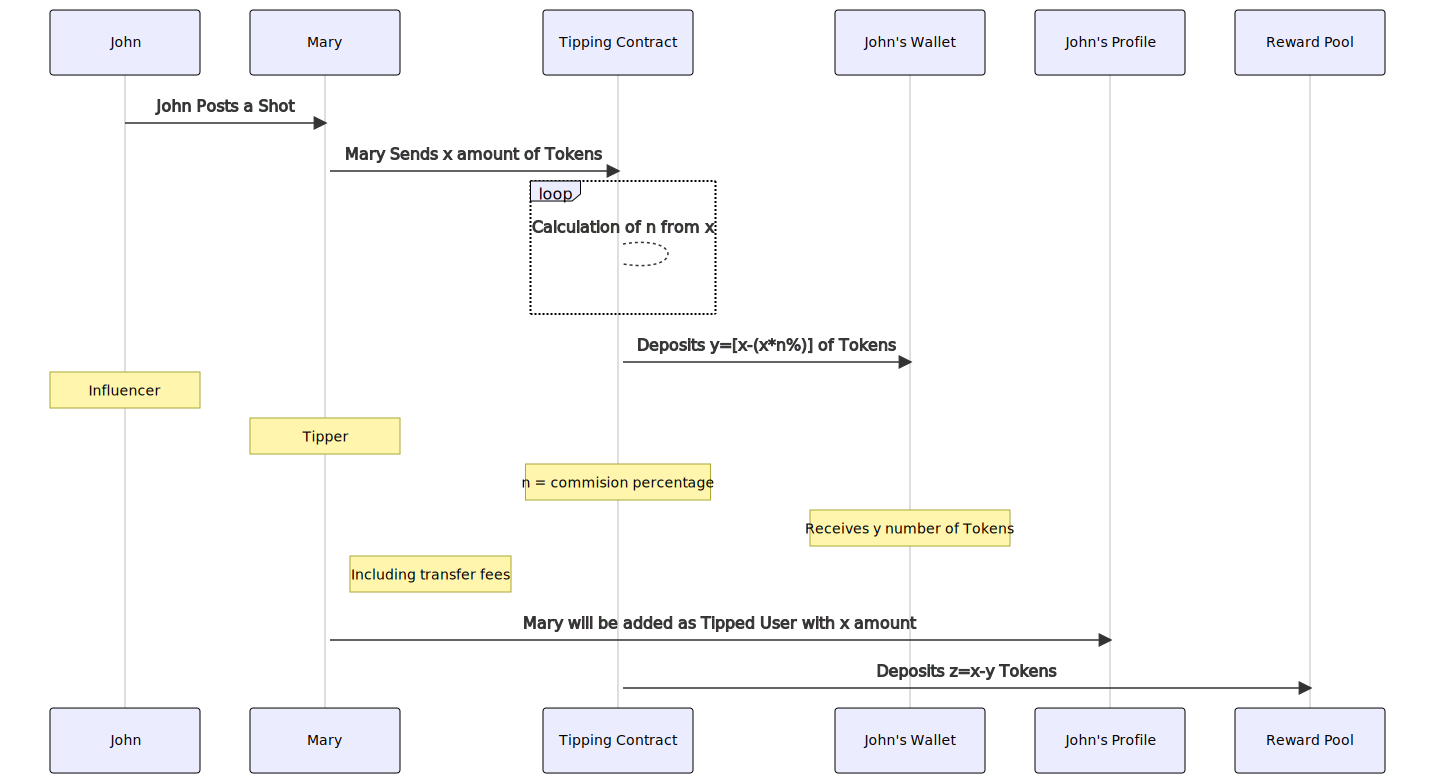
\includegraphics[width=\textwidth]{tips}\\

\begin{lstlisting}[language=Solidity, caption={Tipping Solidity Snippet}]

pragma solidity ^0.8.10;

contract HelloWorld {

    string public greet = "Hello World!";
    
}

\end{lstlisting}

\subsection{Other Features}

\subsubsection{Privacy Groups}

Privacy Groups is a unique feature in Viral to create unlimited friend's groups list to ensure maximum privacy for users to post and share to particular groups of users i.e., Family, Friends, Close Friends, Besties, etc. This feature can empower complete privacy over viewers for certain posts.\\

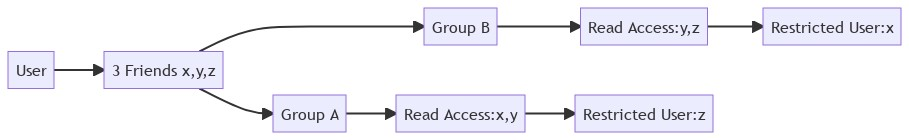
\includegraphics[width=\textwidth]{privacygroups}\\

\begin{lstlisting}[language=Solidity, caption={GunDB Privacy Group Snippet}]

pragma solidity ^0.8.10;

contract HelloWorld {

    string public greet = "Hello World!";
    
}
\end{lstlisting}

\subsubsection{Audio Emoji}

This is a short feature where all the emojis in Viral if touched will give a \textbf{short sound of the emoji}. This will be accessible on chats \& comments section of a post.\\

\subsubsection{Interest Based Recommendation}

To make the viral platform more user-friendly interest-based recommendations are utilized. We have numerous ways to fetch interest from a user \textbf{without collecting data on a centralized server}, a few of them are\\

\begin{itemize}
\item Like \& Dislike
\item Hashtag Follows
\item Search-Based Interests
\item Based on Activity
\item Shares with other friends
\item Following interests
\item Based on Comments
\end{itemize}

All the user interests will be \textbf{stored locally} on the device to ensure \textbf{maximum security} and will be taken to show recommendations.\\

$Flow chart$

\subsection{User Security \& Privacy}

$Abstract$\\

This is classified into\\
\begin{enumerate}
\item Media Storage
\item Chats or Private Messages
\item Interests of User
\item Chat backups
\end{enumerate}

\textbf{1. Media Storage}\\

All Media uploaded to Viral is End-to-end Encrypted where all the files are encrypted using Symmetric AES-256 Encryption Standard on the device and gets uploaded to Trustless IPFS Public Nodes \& Trusted IPFS Cluster Nodes. Thus promising the security of media.\\

\textbf{Encryption}\\

$Detailed Explanation$\\


\begin{figure}

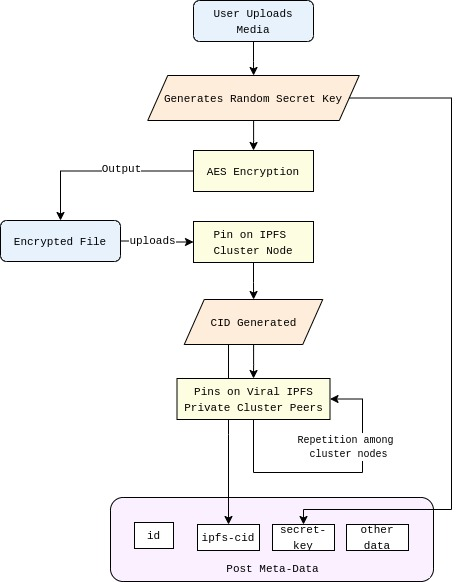
\includegraphics[width=\textwidth]{encryption}\\
\caption{Encryption of Media in Viral}

\end{figure}



\textbf{Decryption}\\

Private Account Media Decryption\\

$Detailed Explanation$\\

\begin{figure}

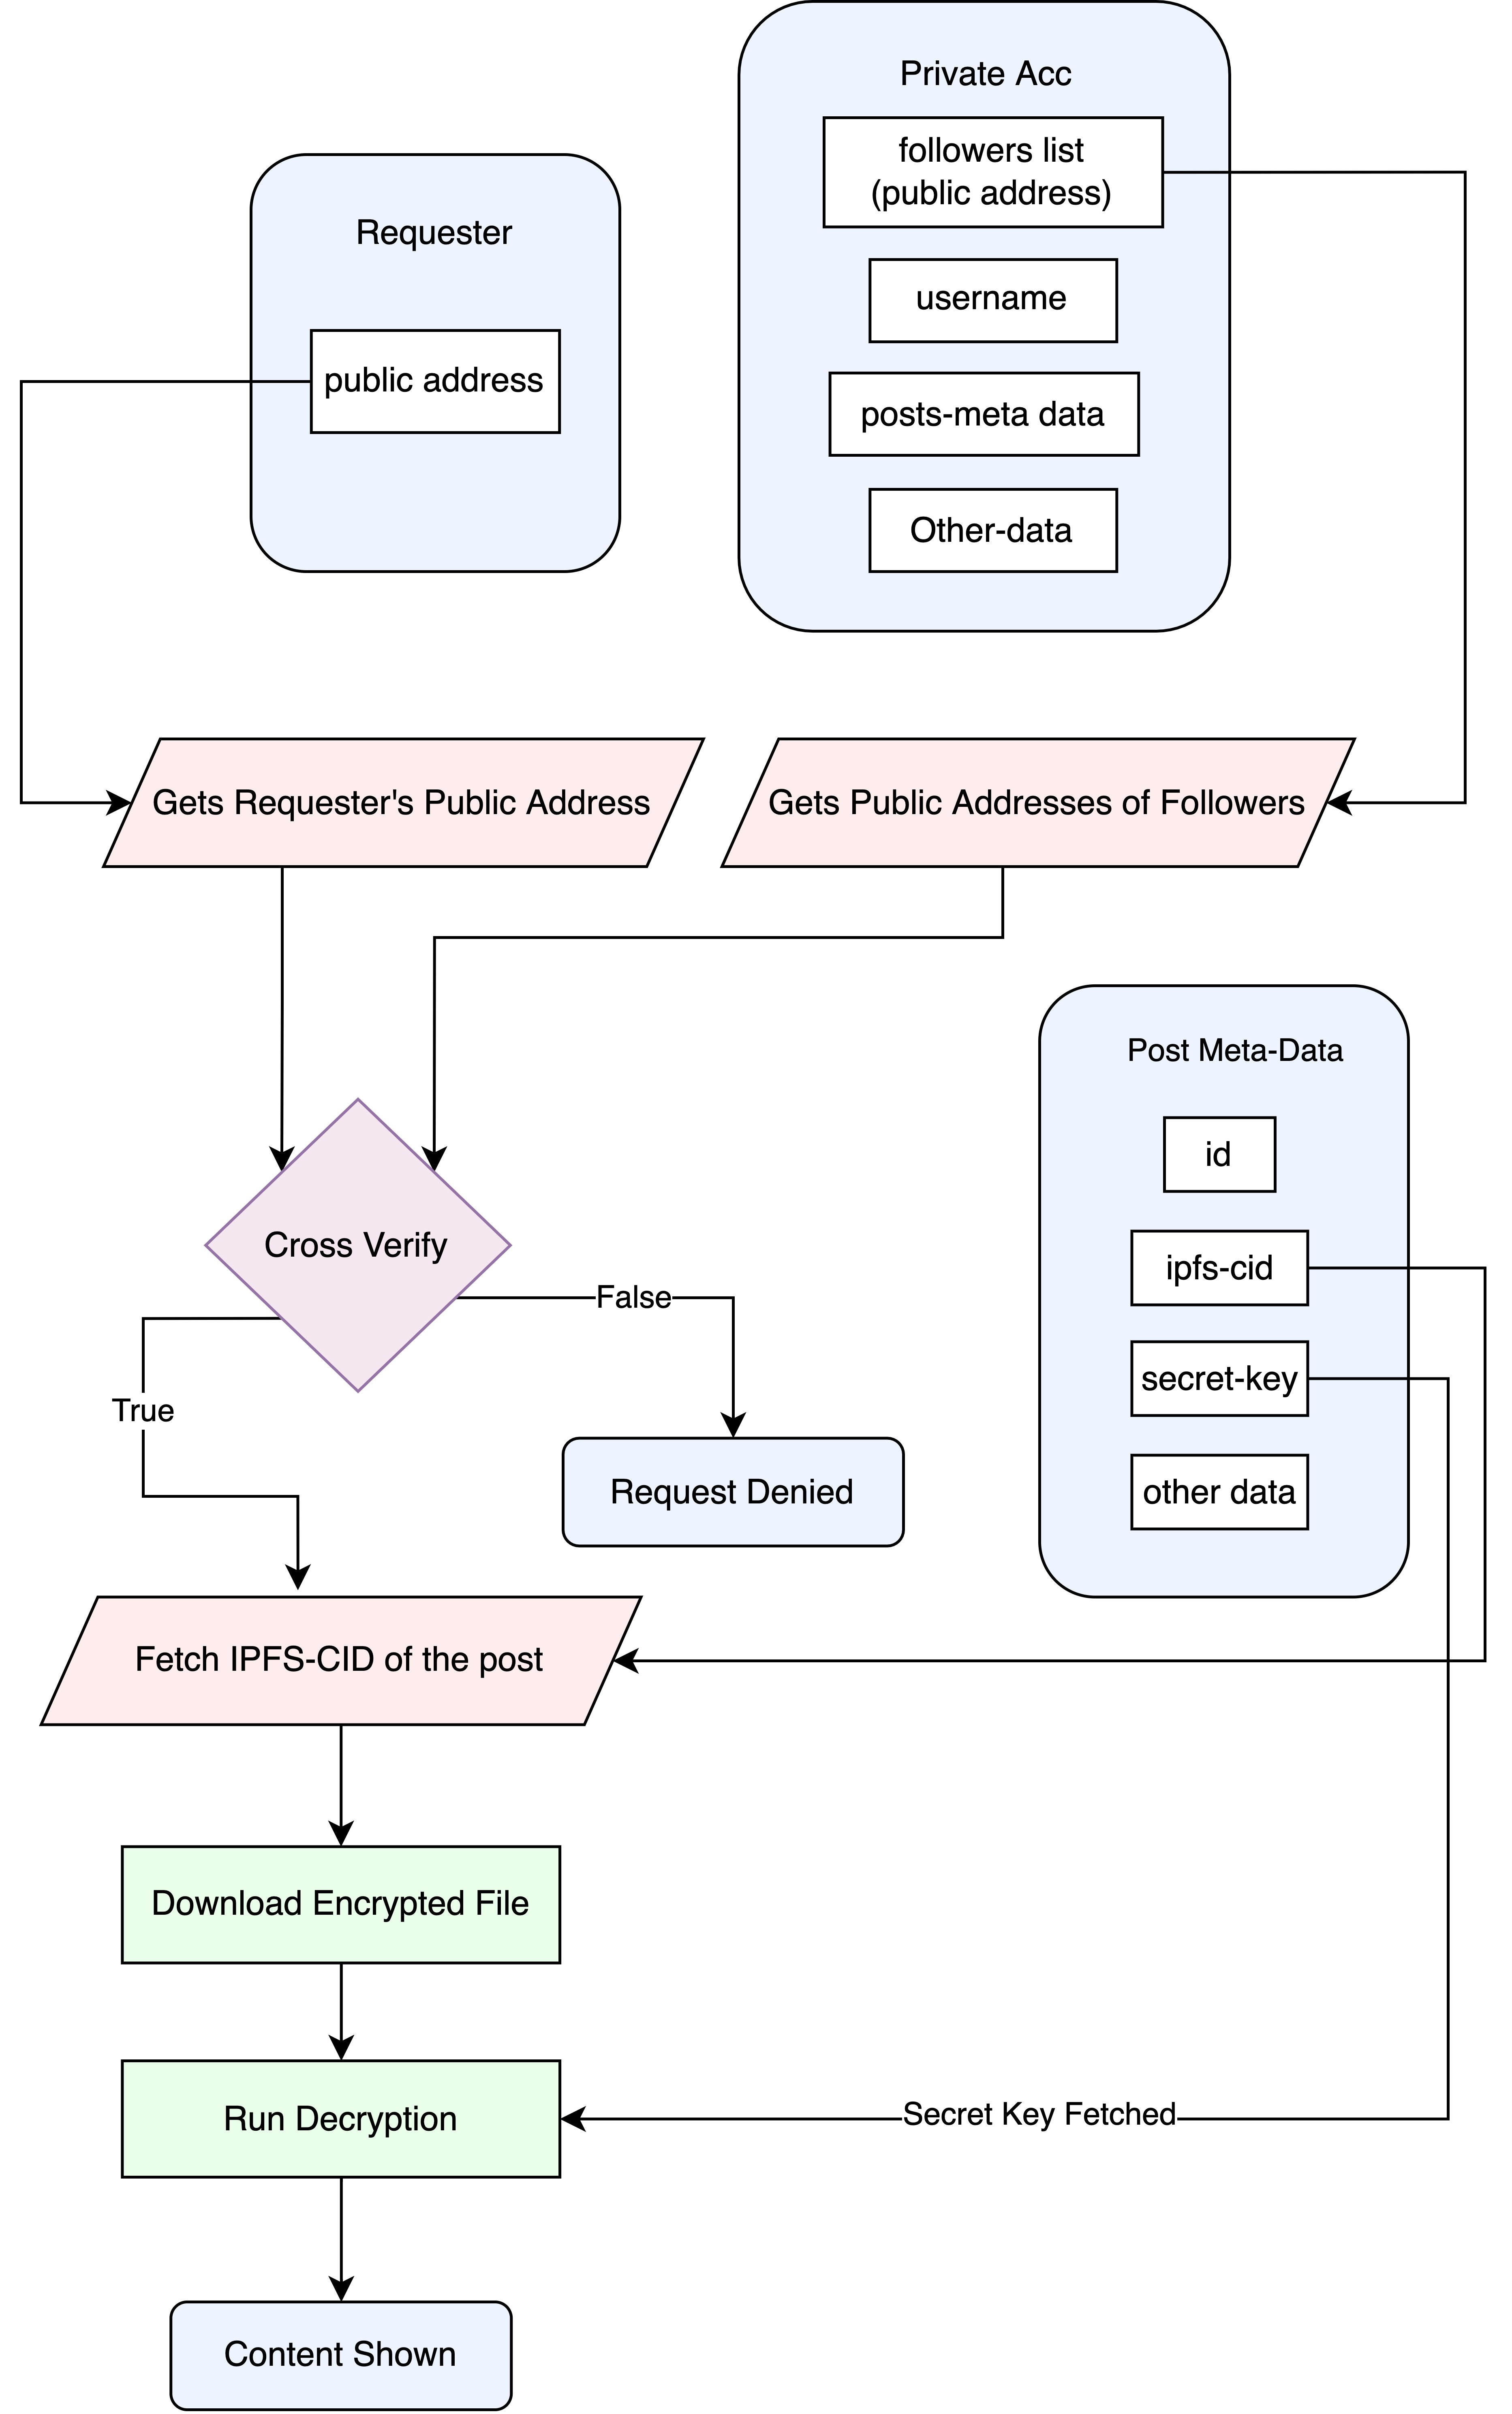
\includegraphics[width=\textwidth]{decryption-private}\\
\caption{Decryption Media of Private account in Viral}

\end{figure}

Public Account Media Decryption\\

$Detailed Explanation$\\

\begin{figure}

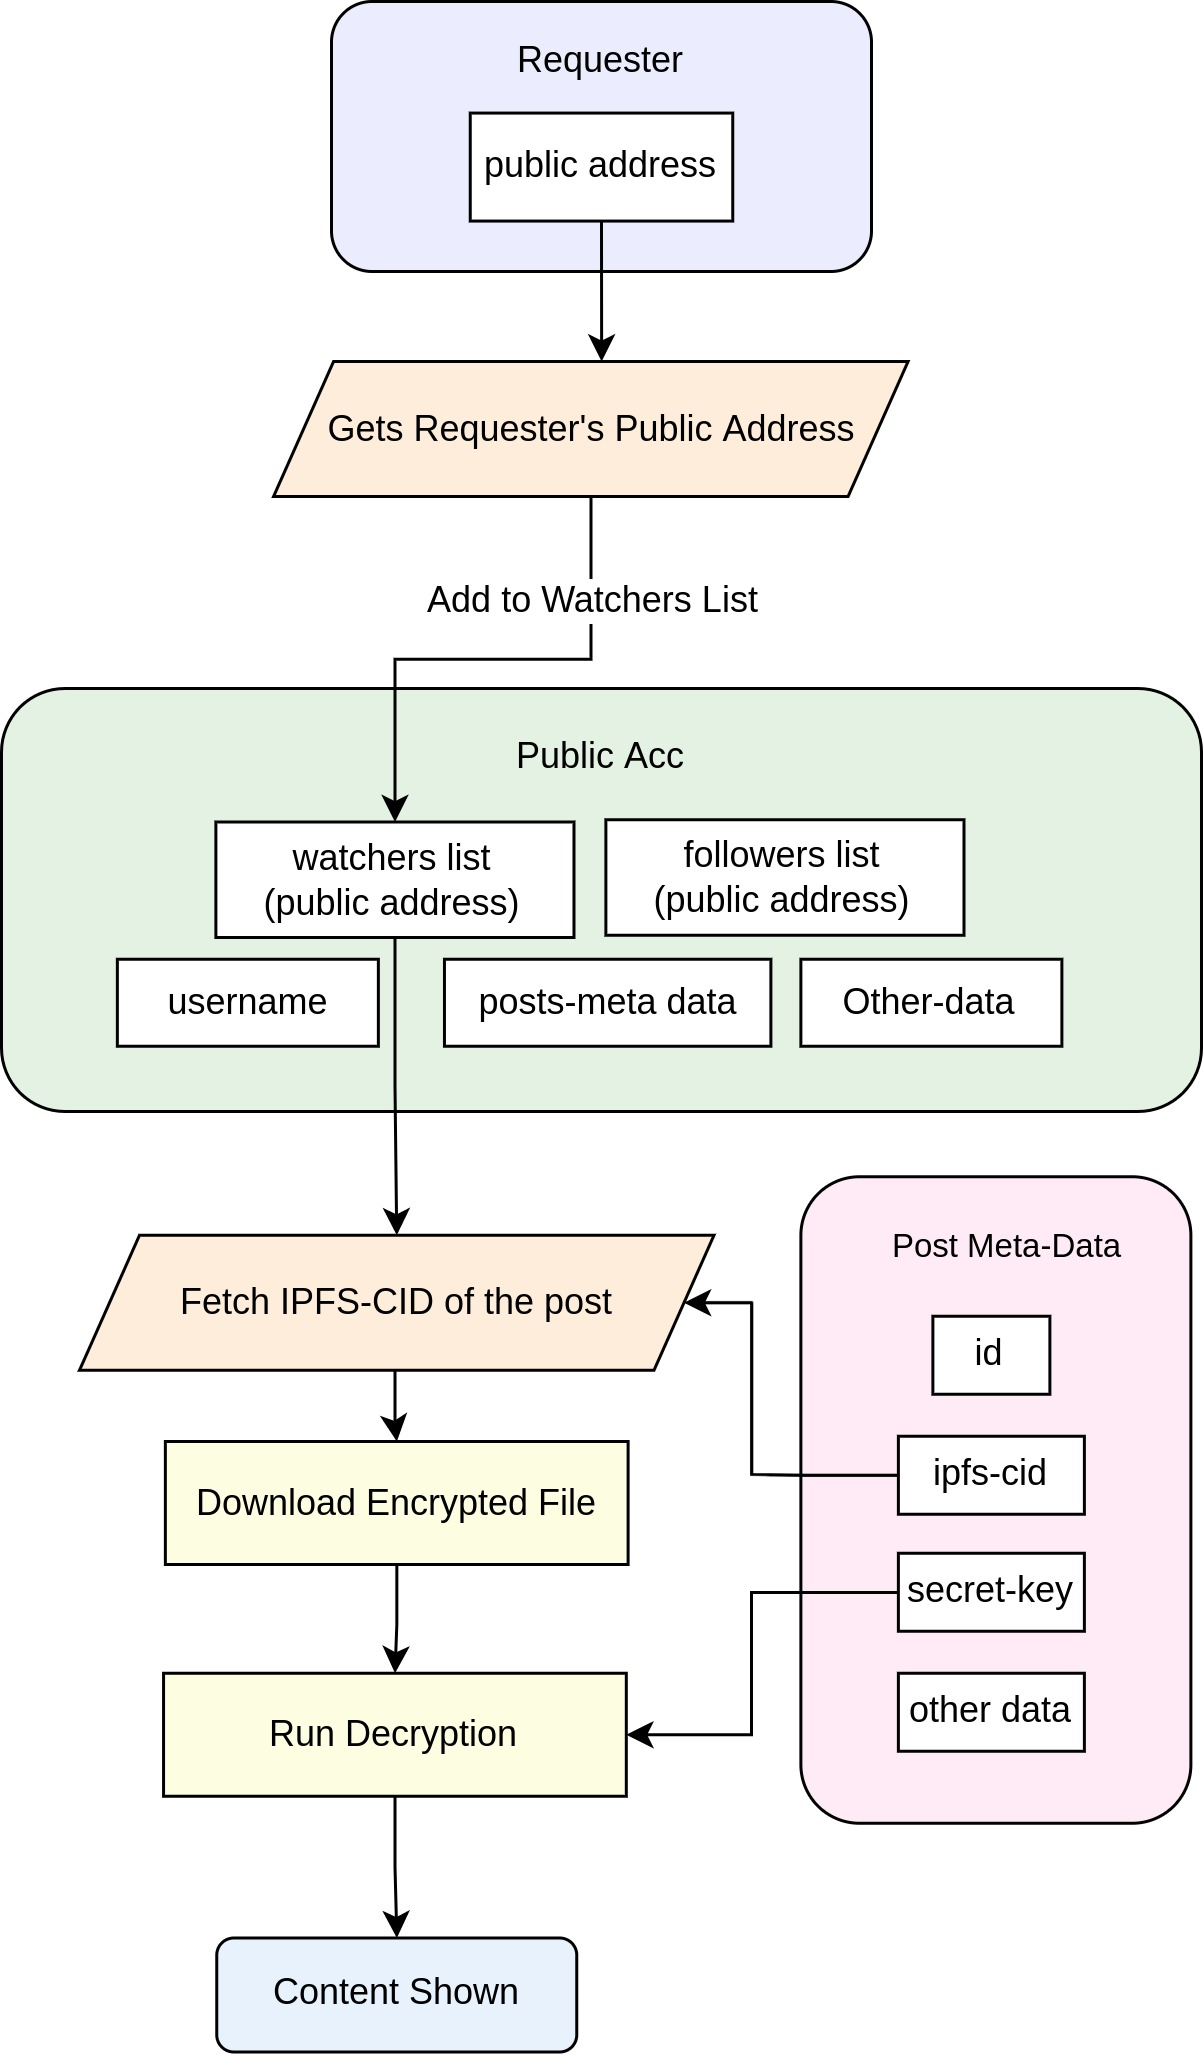
\includegraphics[width=\textwidth]{decryption-public}\\
\caption{Decryption Media of Public account in Viral}

\end{figure}


\textbf{2. Chats \& Private Messages}\\

For Chat-based encryption, Viral uses \textbf{public and private key} encryption method. There are no centralized cloud-based servers involved in storing messages which can potentially trigger breaches. Every single message is encrypted and can be only decrypted by the receiver.\\

Public-Private key encryption more secure than a single shared key which is utilized in multiple chat platforms.\\

$Visual Representation$\\

Alice writes \& Hello \& to Bob – Bob Receives an encrypted message - Bob decrypts using his private key – Bob Sees \& Hello from Alice

\hyperlink{https://sample.com}{GunDB Explanatory Video}\\

\textbf{3. Interests of User}\\

Users' interests will be \textbf{saved locally} on their devices ensuring full privacy of personal data.\\

\textbf{4. Chat Backup}\\

Since Viral is a \textbf{Offline-First Chat} messages will not be stored in cloud. To Backup messages Viral will offer \textbf{cloud options} such as Google Drive/Dropbox where you can securely encrypt and save your \textbf{backup}. While Migrating to another mobile we will be providing a feature to transfer existing messages/interest to your new device.\\

\textbf{Phase 2 Development}\\

We will be focussing on Quantum Resilience of all media encryption used in Viral while commencing the Phase 2 of Development Roadmap\\

\subsection{TOR/VPN Anonymity}

Viral will be a safe haven for anonymity, privacy, and security in eliminating the tracing of users' identities by exploiters . Users can benefit from TOR and VPN Routing Features built in our Decentralized application to hide their IP address and go fully anonymous.\\

TOR routes you through several additional nodes while encrypted, no one can trace it back to you. VPN will redirect your internet traffic through a secure tunnel, hiding your IP address and encrypting your data in the process.\\

\textbf{Content Delivery}\\

Visualization with changes to minting as NFT\\

AES – 256 Encryption Snippet\\

\textbf{IPFS Cluster}\\

Visualization of Repetition\\

Addition of Nodes – Trusted Way\\

Phase 2 – Trust less Way (IPFS-VM)\\

\section{Blockchain, Token Ecosystem and Layer 2}

\subsection{Viral Smart Chain – Short Intro}

Viral Smart Chains, is a network of horizontally scalable EVM Chains on top of IOTA Tangle used for Viral Social network with fully deployed defi ecosystem with Off-Chain solutions. Viral Smart Chains aim to provide an easy understandable one-platform for all the non-crypto users who are subjected to higher gas fees, congestion in network, volatility and scattered defi solutions.\\

\subsection{IOTA Smart Contract Protocol}

IOTA provides an Off-Chain Smart Contract Solution for developers to create multiple-chains on Top of IOTA\textsc{\char13}s immutable Tangle. Since Ethereum transactions are processed On-chain by every single node on its network, it faces additional congestion, slow transaction time and subject to higher miner fees. IOTA\textsc{\char13}s off-chain smart contract solution makes use of blockchains anchored to the Tangle where the smart contracts are ran and achieved consensus with small set of committee nodes. This achieves a high scalable throughput and immutable records since the states of smart contracts such as Account Balances, Input Conditions and Consequences over time are updated on IOTA\textsc{\char13}s Tangle.\\

\textbf{Architecture}\\

$Architecture FlowChart$\\

There are several components to understand more about IOTA\textsc{\char13}s Smart Contracts Protocol. It gives us multi-chain functionality to run smart contracts from different chains which allows a horizontal scaling of blockchains without a need for plasma or side chains.\\

\textbf{Consensus and Validators}\\

IOTA\textsc{\char13}s Smart Contract Chain uses a Byzantine Fault Tolerant \(BFT\) Algorithm, which guarantees consistency and byzantine fault tolerance if less than $1/3$ of nodes are malicious. So the verification process runs on Nodes within a chain committee. With a Proof-of-Stake Consensus each Viral chain will be run by a network of validator nodes, which run a consensus on the chain state updates. The validators of the chain \(Nodes\) form a committee, a bound together closed set of nodes. The committee of the chain can allow new validators and validator nodes to be added or replaced. This also makes the chain itself agnostic to its validators \(the committee\).\\

Viral Smart Chains leverages IOTA Tangle\textsc{\char13}s properties of scalability, high throughput, feeless transactions and immutable records. Only when a supermajority of the validators (the quorum) of a chain reaches consensus, the results get added to the chain where a new state update can be signed, which unlocks the AliasOutput for the chain and produces the next state UTXO which is stored on the Tangle as an immutable record. In summary, the chain\textsc{\char13}s state (data) will be stored on Tangle as an immutable record.The amount of the validators to reach a consensus is configurable for each chain. The committee itself can also be variable in size - from a few nodes up to hundreds of nodes, and each node can be part of many different committees.

\begin{itemize}
\item \textbf{Validators} – Each Single Node running the Chain
\item \textbf{Committee} – The Group of Nodes running a chain
\item \textbf{Quorum} – Number of Nodes to be in consensus to validate a transaction
\end{itemize}

To know more about IOTA\textsc{\char13}s Smart Contracts : \hyperlink{https://files.iota.org/papers/ISC_WP_Nov_10_2021.pdf}{Whitepaper}, \hyperlink{https://wiki.iota.org/smart-contracts/overview}{Documentation}, \hyperlink{https://blog.iota.org/iota-smart-contracts-beta-release/}{Blogs}\\

\subsection{Viral Smart Chains}

Viral Smart Chains are a family of separate chains anchored to the IOTA\textsc{\char13}s Tangle where each chain can communicate with each other via intermediary L1 Value Tangle.\\

\textbf{Viral\textsc{\char13}s Approach}\\

A Single chain will seem complex for setting different fees for different actions on the blockchain i.e Smart Contract Calls/Deployment, Sending Tokens to other Address, etc. Viral\textsc{\char13}s approach is to bring multiple chains categorized by its purpose to serve the Viral Application with fee structure thereby also creating separate chains to provide zero network fees for minting NFTs on Viral App (ERC721 and ERC1155) while rewarding the validators of all Viral chains (including zero fee chains) from the miner pool (total collected fees of all chains) based on validator\textsc{\char13}s total validated transactions for the day through an automated smart contract.\\

\textbf{Validators}\\

Viral Chains will work on Proof-of-stake consensus where validators (miners) are required to stake their Viral Coins in order to participate in the network for validating transactions. The mining power in proof-of stake depends on the amount of coins a validator is staking. Participants who stake more Viral Coins will be most likely to be chosen to add more blocks. When a transaction is validated and attain consensus by the quorum of validators (Read IOTA Protocol), the state of the transaction/smart contract will be recorded in the Value Tangle\textsc{\char13}s UTXO Ledger which makes it immutable. The Transaction will be secured by the validators inside the Viral chain and also the L1 UTXO Ledger.\\

\textbf{Fees}\\

Viral Smart Chain is built primarily to ease the need for gas-based transaction fees like other smart contract blockchains. Transaction fees are only leaved as a fixed percentage as andquot;transfer feeandquot; in Viral Smart Chains for Sending, receiving tokens between accounts and smart contracts.\\

Transfer fees are fixed at 0.05\% of transfer value of the tokens paid in Viral native coin. The minimum fee is capped at \$0.0005 of the fiat value of Viral Coin which is determined using price oracles.\\

$Visualization$\\

Native Token : Bob wants to transfer 100VRL to John : Fee leaved will be 0.05 VRL\\

Other Tokens : If 1 vMATIc = 0.1 VRL\\

Mike wants to transfer 6000 vMATIC to Mia : Fee leaved will be 0.30075 VRL (approx. 3.0075 MATIC) including Swap and Transfer Fee\\

\textbf{NFT Chains}\\

Currently on popular smart contract blockchains such as Ethereum, Polygon the amount of gas required for a transaction is determined by the demand for the transaction to be included, regardless of what type of transaction it is where it is dynamically adjusted based on number of user\textsc{\char13}s interacting with the network at the time.\\

This brings us to an effect that a single blockchain cannot set certain fees or eliminate gas fees for a particular type or category of a transaction regardless of it\textsc{\char13}s nature i.e, smart contract, account transfer. Multiple parallel state blockchains can solve this issue by altering few blockchains as permissioned for a certain use cases and can make it feeless without hindering the other fee-based chains.\\

Viral\textsc{\char13}s aim to democratize NFT to the masses and bring massive NFT Adoption we will be running separate zero-fee chains for deploying ERC721 and ERC1155 Token directly from the Viral Application. The Validators for the chain will be open to join the network where they\textsc{\char13}ll be rewarded from the miner pool (total fee collected) based on the total transactions they validate in a day.\\

\textbf{Family of Chains}\\
\begin{itemize}
\item \textbf{Genesis Chain} : Initialization of First Chain with Viral Coin and Stable Coin Deployment with Smart Contracts that defines governance, fees, etc\\

\item \textbf{General Chains} : For Every n number of active Viral Wallet users a new general chain is deployed. These chains are used to store user funds and create new accounts on the blockchains. So Users can do intra and inter chain transactions with high throughput and flexible scaling.\\
\end{itemize}
\textbf{De-Fi Chains}\\
Smart Contract Deployment Chains specifically for categorized DApps\\
\begin{itemize}

\item \textbf{DEX Chain} : Running smart contracts for Viral Wallet\textsc{\char13}s Decentralized Exchange

\item \textbf{ERC20 Chain} : To Deploy new ERC20 Tokens that can be transacted between chains and accounts

\item \textbf{Viral NFT Chain} : Feeless Viral ran Smart Contract Chain specifically to deploy user\textsc{\char13}s NFTs on-chain

\item \textbf{ERC721/115 Chain} : To deploy new Non-Fungible Tokens for other platforms outside the Viral Application

\item \textbf{Marketplace Chain} : To create smart contract based marketplaces for NFTs and much more

\item \textbf{Other Chains} : For creating Dapps for lending, asset tokenization, yield farming, tools and infrastructure, etc
\end{itemize}

Development

\begin{lstlisting}

      _Root_

      - _Initialization of the chain_
      - _Deployment of new contracts_
      - _Registary of contracts_
      - _Chain ownership management and Access control list_
      - _Fee management_

      _Accounts_

      - _On Chain ledger accounts_
      - _Securely moving tokens between accounts_
      - _Ensuring consistency of the on-chain ledger_

      _Eventlog_

      - _Keeping timestamp immutable log of On-Chain events_

      _Blob_

      - _Keeping registry of Binary objects of arbitrary sizew_

      _Configuration of Committee and quorum_

      _Wasp Nodes_

      _EVM Plugins_

      _Configuring Fees_

      _Smart Contract Deployments_

      _State Updates on Tangle_

      _Multi-Chain Integration_

      _Core-Contracts_

\end{lstlisting}

\subsection{Token Ecosystem}

\textbf{Native Tokens}\\

Viral Coin is the native currency, a digital coin that does all the operations inside the Viral Smart Chains. It is used to store value, send and receive funds within the Multi-Chain Viral Blockchains. Viral Coin is used for paying fees inside the network, staking, governance, rewards and much more.\\

\textbf{Viral Stable Coin}\\

Viral Stable Coin is a sub-native token, an algorithmic stable coin pegged to the US Dollar that is widely used in the Viral Application for sending and receiving tokens across users wallets. Due to constant volatility of the crypto market there is a barrier for the common people and businesses to get into cryptocurrencies. As Viral\textsc{\char13}s aim to become the one-stop crypto solution for the masses we are providing a way for the user\textsc{\char13}s to automatically transact in Stable Coin without any complex need for swapping their current tokens. In Short, when an user transact in Viral Coin, it will force swap and send the receiver viral stable coins to avoid depreciating of the asset while transacting.\\

As far as we know there are several stable coins are in the market 1.Fiat-Peg Centralized, 2.Crypto Collateral 3. Algorithmic. In our case we can take 3 coins 1. USDC 2. DAI 3. AMPL. USDC maintains the peg but holds the funds on its reserves centralized which comes with its demerits. DAI aims to maintain the peg using collateral of several crypto coins, in which USDC hold the reserve of more than 50\% of the DAI\textsc{\char13}s crypto backing, which also makes DAI a centralized cryptocurrency. AMPL is an algorithmic stable coin which maintains it\textsc{\char13}s peg by contracting and expanding it\textsc{\char13}s supply of tokens to achieve stability, this achieves true decentralization but fails to operate swiftly for sudden price movements due to it\textsc{\char13}s rebase function ran in a stipulated time and also rebases in a slow, long way which takes upto a week after a sudden price movement. This is where most crypto projects fail to provide a decentralized stable currency for the masses.\\

Terra blockchain is the most successful running algorithmic stable coin which maintain its stability by changing the stable coin\textsc{\char13}s supply by burning and minting it\textsc{\char13}s native token LUNA. In better words, when Terra (Stable Coin) demand increases to more than \$1, Luna (Native token) will be burned and New Terra tokens will be minted, where increase in supply of tokens resolves the demand and maintains the peg of the stable coin and vice versa. Viral Stable Coin adopts the algorithmic stable coin algorithm used in many of Terra\textsc{\char13}s stable coins.\\

Viral Coin and Viral Stable Coin will be the two primary coins in the Viral Social Platform. The supply and demand of Stable Coin is always balanced by making Viral Coin as it\textsc{\char13}s variable counterweight that absorbs it\textsc{\char13}s volatility.\\

\textbf{1 VSC - \$1 (Expansion)} : When Viral Stable Coin trades at a price that is high relative to it\textsc{\char13}s \$1 peg i.e., \$1.15, the demand for VSC is higher than the circulating supply. To bring the peg back to \$1, the supply of VSC should be increased to balance the demand. During Expansion State trading bots will mint VSC by burning VRL, which has an effect of lowering Viral Stable Coin Price (by expanding the supply) and increases the Viral Coin price (by reducing it\textsc{\char13}s supply). The smart contracts will trade until the price peg of 1 VSC = \$1 is achieved.\\

$Formuka for Expansion$\\

\textbf{1 VSC - \$1 (Contraction)} : When Viral Stable Coin trades at a price that is low relative to it\textsc{\char13}s \$1 peg i.e., \$0.95, the demand for VSC is lower for the circulating supply. To bring the peg back to \$1, the supply of VSC should be decreased to balance the demand. During Contraction State trading bots will burn VSC and mints VRL, which has an effect of increasing Viral Stable Coin Price (by reducing it\textsc{\char13}s supply) and lowering the Viral Coin price (by expanding it\textsc{\char13}s supply). The smart contracts will trade until the price peg of 1 VSC = \$1 is achieved.\\

\textbf{Viral Stable Trading App}\\

High Frequency trading cannot be run using automated smart contracts to maintain price peg of Viral Stable Coin. Users can stake their Coins, run automated arbitrage trading and receive profits using the Viral Stable Trading Application a separate application to maintain the peg of Viral Stable Coin\\

Users will be able to stake both coins VRL and VSC proportionally to a smart contract in the mobile app which process all transactions of burning and minting VRL for VSC automatically without the need for user signature and receive profits from arbitrage opportunities by minting the burning the coins to balance the volatility. The Smart Contracts will add and subtract coins on each pools to maintain stability.\\

\textbf{Viral Bridge}\\











































\end{document}



